\documentclass[12pt, dvipsnames, svgnames, x11names,]{article}

\usepackage{xcolor}
% URLs and hyperlinks ---------------------------------------
\usepackage{hyperref}
\hypersetup{
	colorlinks=true,
	linkcolor=NavyBlue,
	filecolor=magenta,      
	urlcolor=blue,
}
\usepackage{xurl}
%---------------------------------------------------
\usepackage[inline]{enumitem}
\usepackage{graphicx}
\usepackage{multirow}
\usepackage{float}
\renewcommand{\arraystretch}{1.40}

% adjust a verrrrry big table -------------------------------
\usepackage{adjustbox}
% -----------------------------------------------------------

\usepackage{array}
% center the p columns and m --------------------------------------------------------------
\newcolumntype{P}[1]{>{\centering\arraybackslash}p{#1}}
\newcolumntype{M}[1]{>{\centering\arraybackslash}m{#1}}
% -------------------------------------------------------------------------------------------------------------

% price
\usepackage{marvosym}
% ----------

\usepackage{xepersian}
\settextfont{Yas}
\setdigitfont{Yas}

\begin{document}
	\begin{titlepage}
		\centering
		\vspace{1cm}
		{\Huge {\textbf{فرآیند تصمیم مارکوف (MDP)}}\par}
		\vspace{15mm}
		\vspace{16mm}
		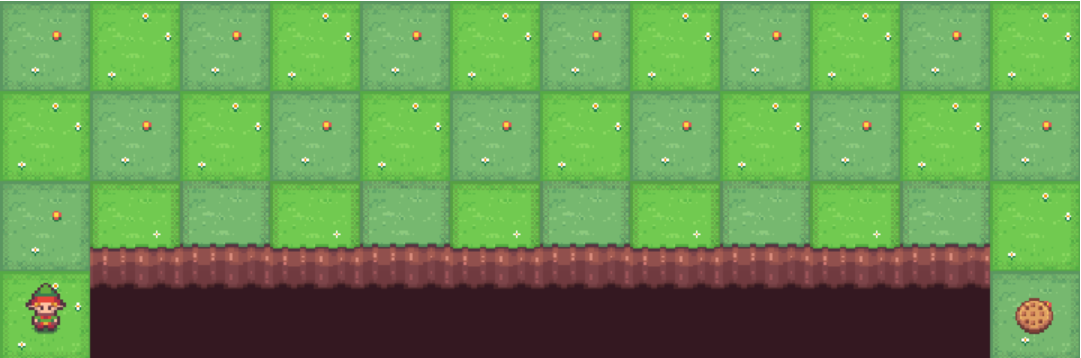
\includegraphics[width=14cm]{images/cliff_walking} \par
		\vfill \par	\vfill
		\vspace{16mm}
		{\normalsize	سیدمحمدحسین هاشمی  4022363143 \par}
		
		{\normalsize	سیدحسین حسینی  4012363238 \par}
		\vspace{1cm}
		{\large آبان ۱۴۰۲\par}
	\end{titlepage}
	\tableofcontents
	\newpage
	
	
	\section{لیست صخره ها}
	
		{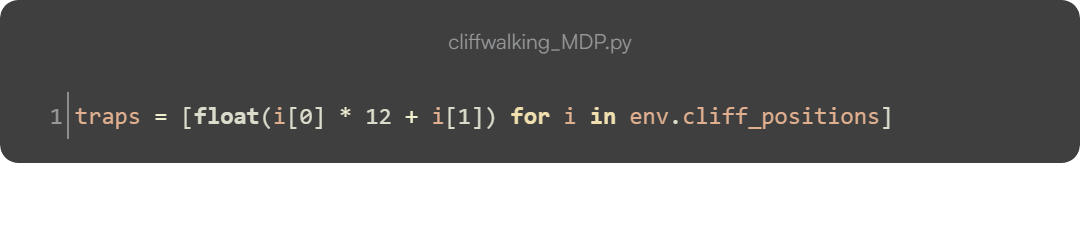
\includegraphics[width=14cm]{images/01}}
		{\normalsize شماره خانه های صخره درون لیست \lr{traps} ذخیره می‌شود.}
		
	\section{آماده سازی دیکشنری \lr{states}}
	
		{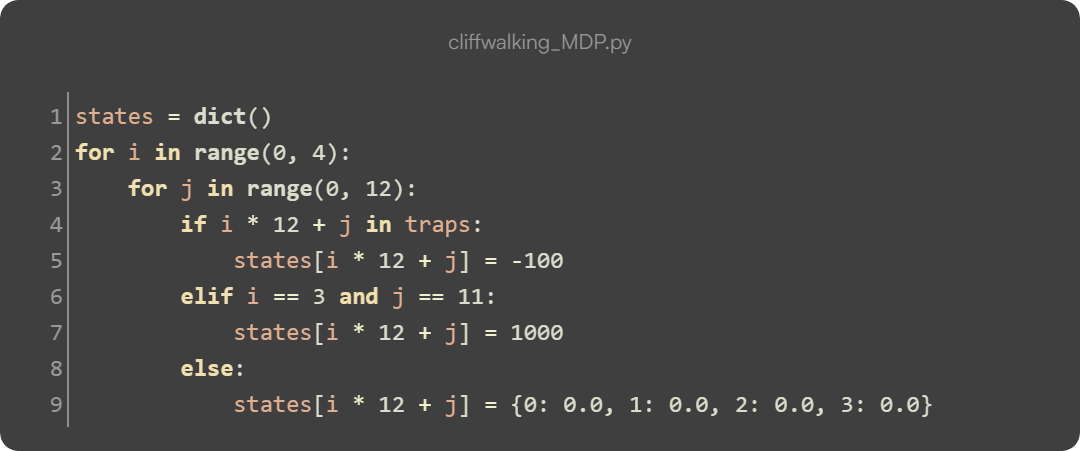
\includegraphics[width=14cm]{images/02}}
		{\normalsize از دیکسشنری \lr{states} برای محاسبات استفاده می‌کنیم.}
		{\normalsize در اینجا مقادیر اولیه آن را تعریف کرده‌ایم.}
	
		
	\section{تابع محاسبه امتیاز خانه}
	
		{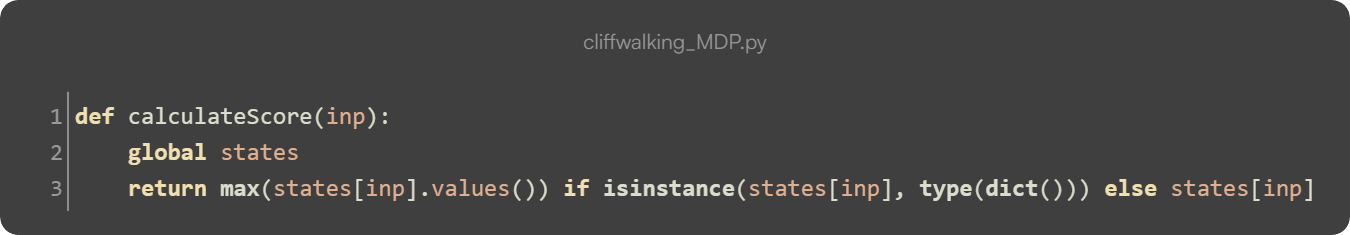
\includegraphics[width=14cm]{images/03}}
		{\normalsize این تابع ارزش خانه فراخوانی شده را برمی‌گرداند. بدین صورت که در صورت بودن هدف و یا صخره مستقیما امتیاز آن برگشت داده می‌شود و در غیر اینصورت مقدار بیشترین عمل برگشت داده می‌شود.}
	
		
	\section{تابع به روز کردن ارزش عمل}
	
		{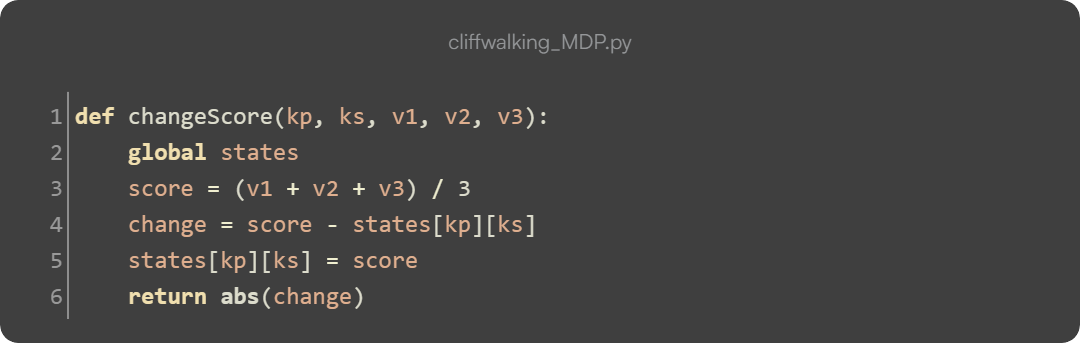
\includegraphics[width=14cm]{images/04}}
		{\normalsize از این تابع برای بروز مقدار ارزش هر عمل استفاده می‌شود و مقدار بازگشت داده شده مقدار تغییرات آن است.}
		
	\newpage
	\section{تابع بروز کردن مقادیر \lr{states}}
	
		{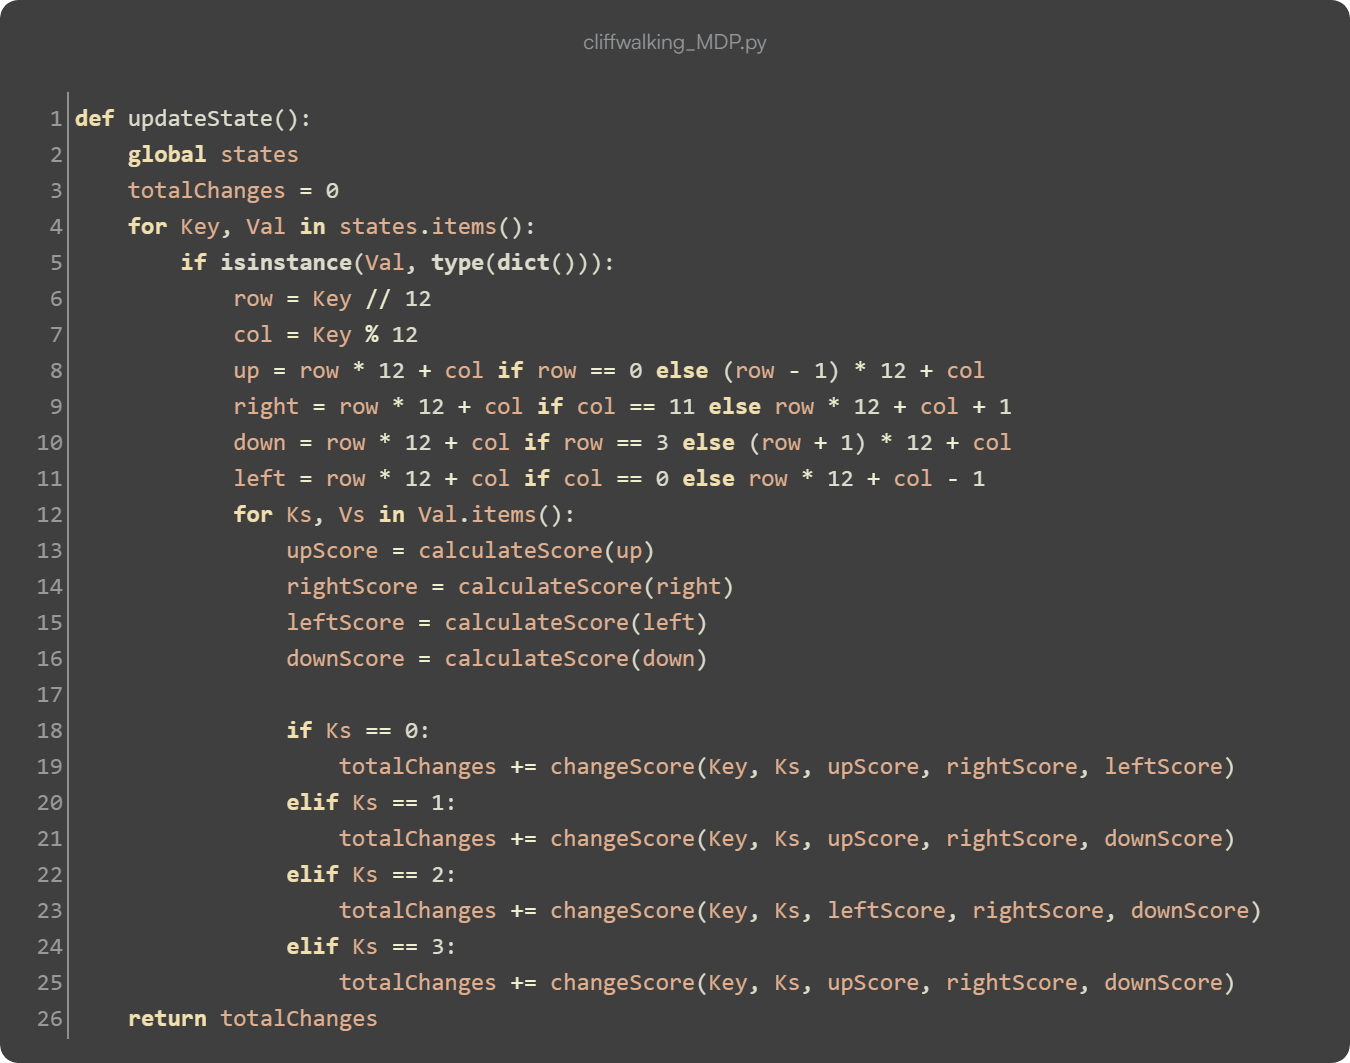
\includegraphics[width=14cm]{images/05}}
		{\normalsize این تابع اصلی برای بروز کردن مقادیر \lr{states} است.} \par
		{\normalsize بدین صورت که با هر بار اجرا بصورت مستقل عمل می‌کند و  هر احرای آن هر خانه و عمل‌های آن را ارزش‌گذاری و مقدار کل تغییرات را برمی‌گرداند.} \par
		{\normalsize پس از پیمایش \lr{states} درصورتی که خانه صخره و یا هدف نبود، موقعیت بعدی آن را از هر سمت به دست می‌آوریم و سپس امتیاز اعمال را با استفاده از توابع بالا بروز رسانی می‌کنیم.} \par
	
		
	\section{حلقه مارکوف}
	
	{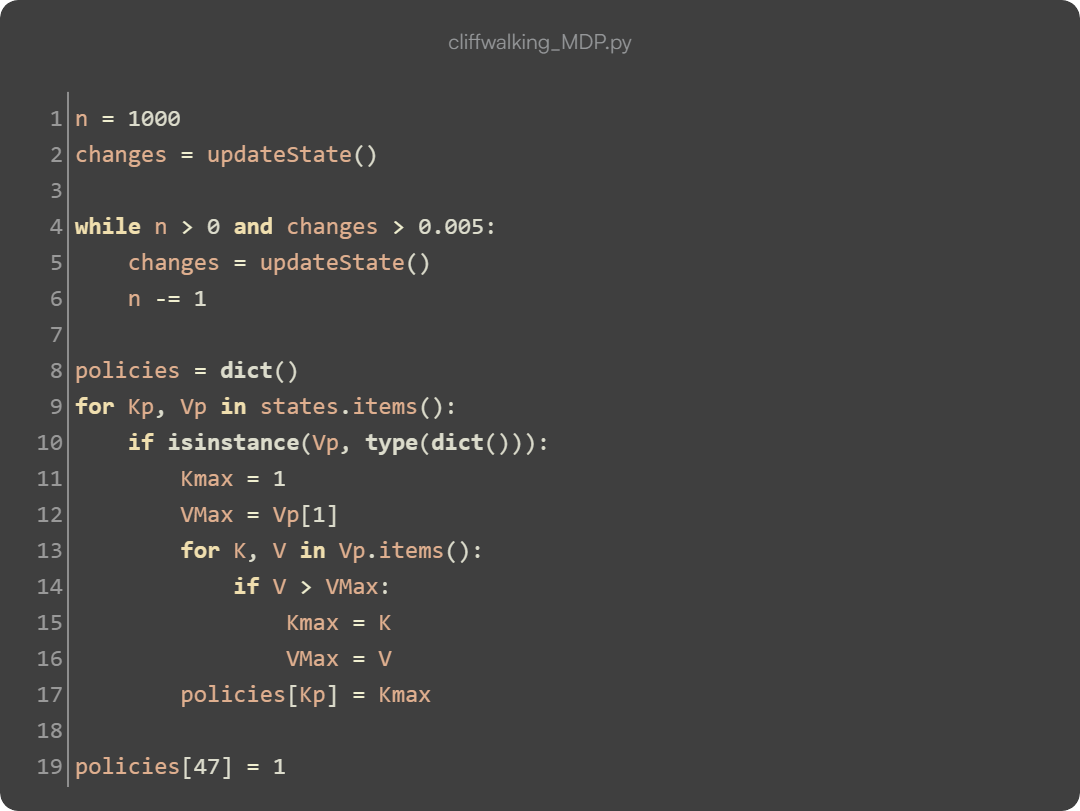
\includegraphics[width=14cm]{images/06}}
	{\normalsize این حلقه همان حلقه معروف فرایند مارکوف است که در صورت کم نشدن مقدار تغییرات هزار بار تابع \lr{updateState} را فراخوانی و مقدار \lr{states} را بروز می‌کند.} \par
	{\normalsize بعد از آن \lr{policies} را با استفاده از \lr{states} ایجاد کرده‌ایم، بدین صورت که با ارزش ترین عمل انتخواب می‌شود.} \par
	{\normalsize در نهایت برای اینکه خانه 47 خانه هدف است حساب نشده که برای رفع باگ مقدار 1 (حرکت به راست) را برای آن قرارداده‌ایم.}

	
		
	\section{لیست صخره ها}
	
	{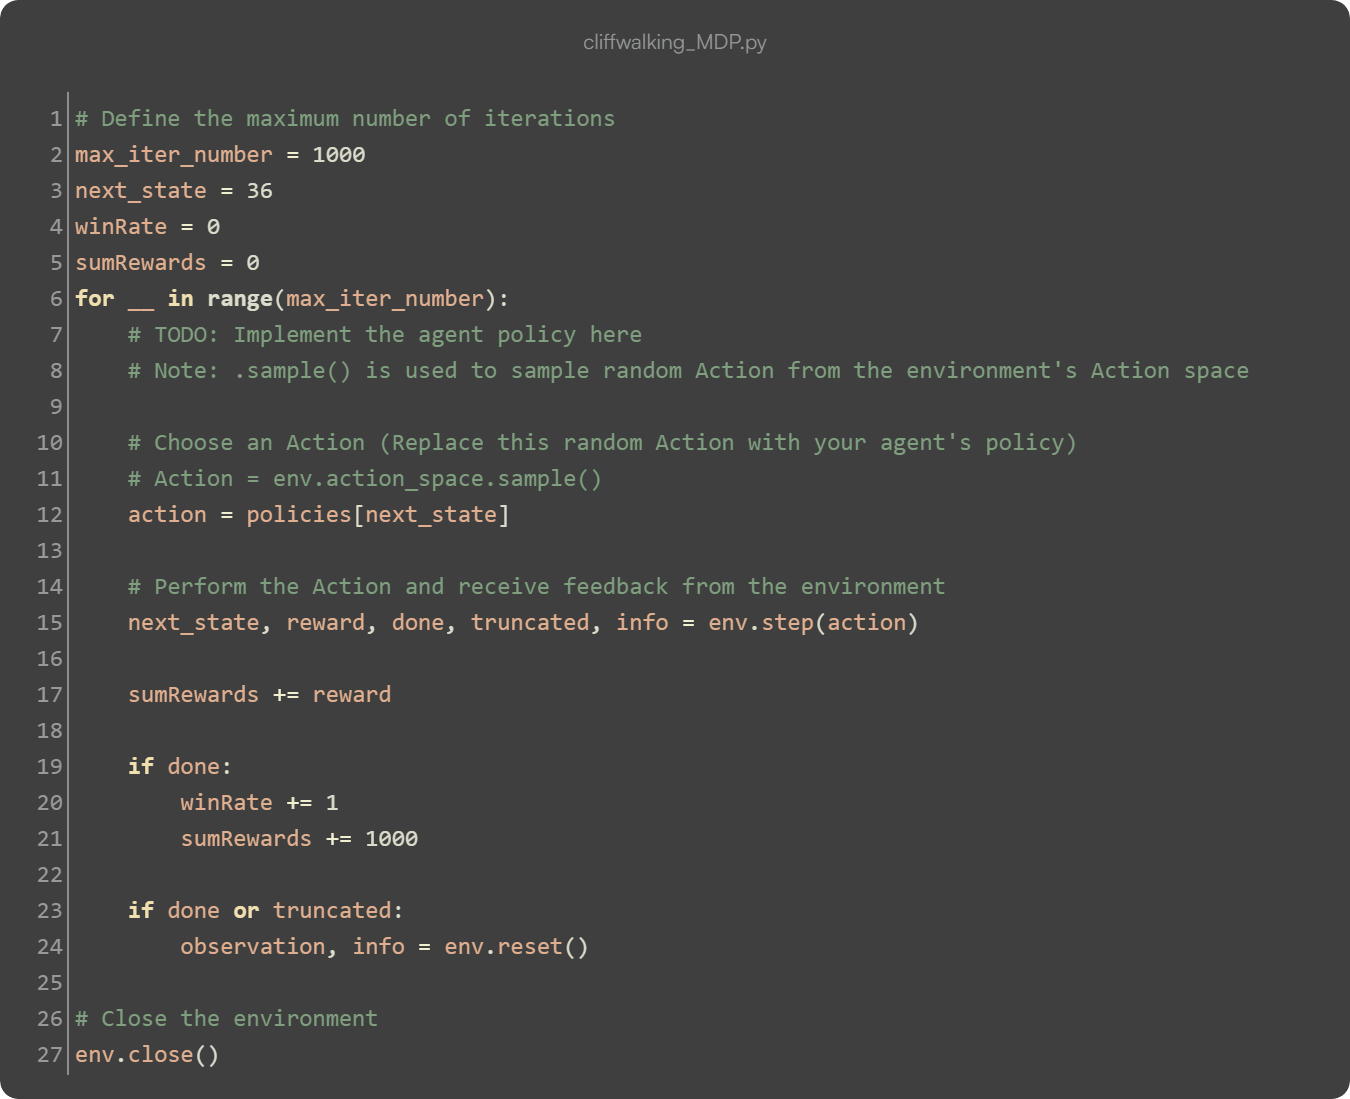
\includegraphics[width=14cm]{images/07}}
	{\normalsize با قرار دادن \lr{policies} در کد کار به اتمام می‌رسد. } \par

	
\end{document}